\documentclass[10pt,a4paper]{article}
\usepackage[utf8]{inputenc}
\usepackage[french]{babel}
\usepackage[T1]{fontenc}
\usepackage{amsmath}
\usepackage{amsfonts}
\usepackage{amssymb}
\usepackage{graphicx}

\usepackage{libertine}
\setlength{\parindent}{0cm}
\setlength{\parskip}{1ex plus 0.5ex minus 0.2ex}
\newcommand{\hsp}{\hspace{20pt}}
\newcommand{\HRule}{\rule{\linewidth}{0.5mm}}

\begin{document}

\begin{titlepage}
  \begin{sffamily}
  \begin{center}

    % Upper part of the page. The '~' is needed because \\
    % only works if a paragraph has started.
    
\includegraphics[scale=0.15]{images/tree.jpg}~\\[1.5cm]

    \textsc{\LARGE U-MONS}\\[2cm]

    \textsc{\Large Rapport de projet de Structures de données 2}\\[1.5cm]

    % Title
    \HRule \\[0.4cm]
    { \huge \bfseries Priority Search Tree and Windowing\\[0.4cm] }

    \HRule \\[2cm]
    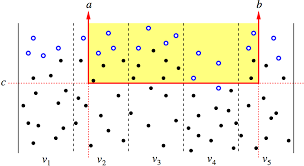
\includegraphics[scale=0.50]{images/window.png}
    \\[2cm]

    % Author and supervisor
    \begin{minipage}{0.4\textwidth}
      \begin{flushleft} \large
        \emph{\textbf{Directeurs :}}\\ G.Devillez et V.Bruyère\\
      \end{flushleft}
    \end{minipage}
    \begin{minipage}{0.4\textwidth}
      \begin{flushright} \large
        \emph{\textbf{Groupe :}}\\ M.Salemi et A.Lecocq
      \end{flushright}
    \end{minipage}

    \vfill

    % Bottom of the page
    {\large \today}

  \end{center}
  \end{sffamily}
\end{titlepage}

\newpage
\tableofcontents
\newpage
\section{Introduction}
Dans le cadre du cours de structures de données 2, nous avons été amenés à réaliser un projet en Java. Ce projet a pour objectif de créer et manipuler une structure de données non vue au cours. Cette nouvelle structure se base sur un arbre de recherche à priorité (Priority Search Tree en anglais ou PST). De la documentation nous a été fournie afin de nous familiariser avec cette dernière structure qui elle non plus n'a pas été vue au cours.

\section{Priority Search Tree}

\subsection{Objectif de la structure}
Un PST est une structure de données de type arbre binaire (chaque nœud comporte au plus deux fils). Cette structure de données organise des points de l'espace défini par deux coordonnées X et Y. L'organisation des données permet d'effectuer efficacement la recherche des points présents dans une fenêtre de l'espace (sans avoir à parcourir l'ensemble des points).

\subsection{Définition}
Un PST correspond à une structure de données mixte. Chaque nœud est constitué d'un point et d'un nombre appelé la médiane. Si l'on considère uniquement les coordonnées X, un PST est un tas avec le minimum à la racine. Le tas ayant été vu en profondeur au cours, nous n'en parlerons pas d'avantage. Si l'on considère maintenant uniquement les coordonnées Y, le PST est un arbre de binaire de recherche avec une petite particularité. Au lieu de trier les fils par rapport à la donnée du nœud courant, un PST trie les fils en fonction de la médiane du nœud courant. Ainsi, tout nœud n d'un PST respecte les contraintes suivantes :
\begin{itemize}
	\item son fils gauche (s'il existe ainsi que ses descendants s'ils existent) aura sa coordonnée X plus grande que celle du nœud n et sa coordonnée Y plus petite que la médiane du nœud n ;
	\item son fils droit (s'il existe ainsi que ses descendants s'ils existent) aura sa coordonnée X plus grande que celle du nœud n et sa coordonnée Y plus grande que la médiane du nœud n.
\end{itemize}

\subsection{Construction}
La construction d'un PST est assez simple si l'on construit ce dernier à partir d'une liste de points triés avec la coordonnée Y strictement croissante. Nous avons vu au cours que ce tri peut être obtenu en complexité O(n). Le PST se construit récursivement. Nous construisons la racine à partir de la liste de points triés. Pour construire un nœud à partir d'une liste de points triés, recherchons le point avec la plus petite coordonnée en X [complexité O(n)] et supprimons le de la liste. Attribuons ce point au nœud courant. De cette manière, nous sommes sûr que tous les fils de ce nœud auront une coordonnée en X plus grande. Séparons le reste de la liste en deux 
% TODO continue ...

\subsection{Windowing}
Le windowing est une technique très répandue qui consiste à sélectionner certaine une fenêtre parmis une énorme quantité de données. Un exemple pratique très répandu est l'affichage d'une carte sur un gps, le gps se voulant rapide n'affichera pas toutes les routes qui se trouvent dans le monde(énorme quantité de données) mais seulement celles qui nous entourent au moment où  nous roulons avec notre véhicule. 

\subsection{Mise en place du problème}
Pour ce projet, il nous été demandé de résoudre un problème de windowing utilisant la structure de donnée "Priority Search Tree". Il nous est donc fourni un fichier.txt qui contient un ensemble de segments que nous devons pouvoir afficher et sélectionner à travers la dite technique. \\
Il faut donc pouvoir gérer différents type de fenêtres lors du windowing :
\begin{enumerate}
	\item \begin{Huge}
	À remplir
	\end{Huge}
	\item 
	
\end{enumerate}

\section{Idées et Mise en pratique}
\section{Diagramme de Classes}
\section{Algorithmes et explications}

\section{Illustrations}

\section{Conclusion}


\end{document}